\documentclass{article}
\usepackage[preprint]{neurips_2025}   % official NeurIPS 2025 style (2026 not published at build time)
\usepackage[utf8]{inputenc}
\usepackage[T1]{fontenc}
\usepackage{hyperref}
\usepackage{url}
\usepackage{booktabs}
\usepackage{amsfonts,amsmath}
\usepackage{nicefrac}
\usepackage{microtype}
\usepackage{xcolor}
\usepackage{graphicx}
\usepackage{capt-of}

% Every number in Results comes from a file generated by paper/figs/make_figs.py from results/. Never type one in.
\newcommand{\todo}[1]{\textcolor{red}{[TODO: #1]}}
\newcommand{\pythia}[1]{Pythia-#1}

\title{How Many Canaries Does a Writer Need?\\Auditing Training-Data Use with Planted Canaries}

\author{%
  Manas Ganti \And Teammate 2 \And Teammate 3 \\
  Virginia Tech \\
  \todo{names, emails}
}

\begin{document}
\maketitle

\begin{abstract}
% Headline numbers from paper/tables/scorecard.md and table1_bundle.tex.
Writers have no reliable way to show that a language model was trained on their work: membership-inference
attacks are close to random on large models when members and non-members come from the same distribution. We
study a creator-side alternative, \emph{canaries}: hidden, made-up details that a writer plants in their text and
later tests for. We ask how many copies of which canary a writer needs before training on their work becomes
provable at $p<0.01$, and with what access. We continue pretraining \pythia{160M} and \pythia{410M} on Wikipedia with four canary
types (random sequences, fluent trap sentences, invisible-character watermarks, and fictional facts) planted at
1, 4, 16 or 64 copies, with matched never-planted canaries as controls, and pass the corpus through realistic
cleaning steps (substring deduplication, Unicode normalization, paraphrasing). A pre-registered one-sided
Mann--Whitney test on member vs.\ non-member scores gives exact false-positive control, which we verify on the
untouched base models (0 of 32 tests significant at each size). With log-probability access, the larger model
detects every canary type from a single copy, but only when repeated canaries of the same kind are also in the
corpus: once deduplication removes those repeats, the same single copies are barely detectable. Unicode
normalization strips watermarks, and substring deduplication removes every verbatim canary type. Only fictional
facts, phrased differently in each copy, survive all three cleaning steps (16 copies for a 25-fact bundle on
\pythia{410M}). With text-only access, verbatim canaries become detectable from 4 copies on the larger model, but
fictional facts are never reliably detected.

\end{abstract}

\section{Introduction}
Large language models are trained on web-scale text whose authors were rarely asked. A writer who suspects their
work was used has few options: training corpora are undisclosed, and post-hoc membership-inference attacks (MIAs)
perform close to chance on large models once members and non-members are drawn from the same distribution
\citep{duan2024membership,das2024blind}, so they cannot support an accusation
\citep{zhang2024membership}. A more promising route is for the creator to act \emph{before} publication: plant
\emph{canaries}, unique strings with no reason to appear elsewhere, and later test whether a model has memorized
them \citep{carlini2019secret,meeus2024copyright,wei2024proving}.

The practical question is quantitative. A writer controls how many canaries they plant and what they look like,
but not how the developer's pipeline treats them: deduplication can remove repeats, Unicode normalization can
erase invisible marks, and paraphrasing can destroy verbatim strings. Nor does the writer control the access they
get: commercial models usually expose text, not log-probabilities. We therefore ask:
\textbf{how many copies of which canary does a writer need before training on their work becomes provable, and
with what access?}

We answer with a controlled study in which ground truth is known. We continue pretraining \pythia{160M} and \pythia{410M}
\citep{biderman2023pythia} on Wikipedia into which we plant canaries of four types at four copy counts; matched
canaries from the same generators that are never planted serve as non-members, and the member/non-member split
is randomized after generation, which makes a rank test of member vs.\ non-member scores a valid permutation-style
test with exact false-positive control. Our contributions:
\begin{itemize}
  \item A \textbf{canary scorecard} (Table~\ref{tab:scorecard}): for each canary type, the minimum number of copies
        detectable at $p<0.01$, whether it survives deduplication, normalization and paraphrasing, whether
        text-only access suffices, and its false-positive rate on a model that never saw it.
  \item \textbf{Dose--response and survival measurements} under realistic pipelines and two access levels
        (Figures~\ref{fig:dose} and~\ref{fig:survival}) at two model sizes, including the finding that single copies are only detectable when repeated canaries of the same kind are also present.
  \item A \textbf{pre-registered audit protocol} whose false-positive control we verify empirically on the clean
        base models (Appendix~\ref{app:qq}), and released code that turns the protocol into a tool for creators.
\end{itemize}

\section{Related work}
\textbf{Membership inference on LMs.} Loss-based attacks \citep{carlini2021extracting}, Min-K\% \citep{shi2024detecting}
and Min-K\%++ \citep{zhang2025minkpp} score how unusually likely a text is under the model. Evaluations with
same-distribution non-members find these attacks near chance on large pretrained models
\citep{duan2024membership,das2024blind}, and \citet{zhang2024membership} argue that MIAs cannot, in principle,
prove that a model was trained on given data without a randomized control. Dataset inference aggregates weak
signals over many documents \citep{maini2024llm}; our test does the same over a creator's bundle of canaries.

\textbf{Canaries, traps and data watermarks.} \citet{carlini2019secret} introduced random canaries to measure
unintended memorization. Copyright traps \citep{meeus2024copyright} plant repeated fictitious sequences in
documents; \citet{shilov2024mosaic} show fuzzy duplicates are memorized almost as well as exact ones.
\citet{wei2024proving} plant random-sequence and Unicode watermarks and test with a hypothesis test against
re-sampled watermarks, which is the closest design to ours. \todo{verify STAMP, radioactive watermarks, and any
2025--26 work on canary survival under cleaning/post-training (CLAUDE.md §10); adjust contributions if needed.}

\textbf{Deduplication and memorization.} Deduplication reduces memorization \citep{lee2022deduplicating,kandpal2022deduplicating},
which is exactly what threatens repeated canaries. Facts are learned from varied mentions rather than verbatim
repetition \citep{allenzhu2023physics}, which motivates our paraphrased fictional facts.

\section{Threat model and audit test}\label{sec:threat}
\textbf{Parties.} A \emph{creator} publishes text containing canaries. A \emph{developer} collects it and trains a
model after a data pipeline the creator does not control (deduplication, normalization, paraphrasing). An
\emph{auditor} acting for the creator queries the model with either \emph{gray-box} access (per-token
log-probabilities of a given text) or \emph{black-box} access (sampled text only).

\textbf{Randomized controls.} The creator generates $2m$ canaries from one generator and, \emph{after} generation,
splits them at random into $m$ members that are published and $m$ non-members kept secret. If the model never saw
the creator's text, member and non-member scores are exchangeable, so any rank test on them has its nominal
false-positive rate regardless of how good or bad the detector is. This is what lets a weak per-canary signal
support a strong, calibrated claim \citep{zhang2024membership}.

\textbf{Test.} For a detector score $s$ (oriented so that higher means more member-like), we compute a one-sided
Mann--Whitney $U$ test of $H_0$: members and non-members are exchangeable, against the alternative that members
score higher, and reject at $\alpha=0.01$. We pre-registered one primary detector per access level
(Appendix~\ref{app:prereg}): gray box uses the mean token log-likelihood (\emph{loss}); black box uses
\emph{completion}, the fraction of a canary's second half reproduced by greedy decoding from its first half (for
fictional facts: the fraction of 16 samples from a held-out question phrasing that produce the answer). We report
AUC, TPR at 1\% FPR, and the minimum bundle size $m$ at which $\ge 80\%$ of resampled bundles reach $p<0.01$.

\section{Canary designs}\label{sec:canaries}
All four generators are seeded and produce unlimited distinct canaries (\texttt{canary/generate.py}); examples are
in Appendix~\ref{app:examples}.
\begin{itemize}
  \item \textbf{Random sequence}: 24 random alphanumeric pseudo-words (about 70--110 tokens). Maximally surprising,
        so easy to memorize, but trivially flagged by quality filters.
  \item \textbf{Fluent trap}: template-generated English sentences with random fills, at least 44 words
        (${\ge}47$ tokens), copied verbatim. Fluent, but every copy is identical, so substring deduplication can
        remove repeats.
  \item \textbf{Invisible watermark}: a fluent carrier passage in which about 30\% of words are followed by a
        zero-width character (Unicode category Cf) and about 20\% of eligible Latin letters are replaced by
        Cyrillic homoglyphs. Invisible to readers.
  \item \textbf{Fictional fact}: an invented entity with one relation whose answer comes from a closed answer
        space (``The Varnholt Bridge opened in 1847''; years 1700--1949 or one of 60 cities). Each planted copy uses
        a different one of eight phrasings, as real authors vary their wording; the audit asks a ninth phrasing
        that is never planted, so detection requires extracting the fact, not recalling a string.
\end{itemize}
Verbatim canaries are at least 47 tokens long so that the 50-token substring deduplication of
\citet{lee2022deduplicating} can, in principle, catch their repeats.

\section{Experimental setup}\label{sec:setup}
\textbf{Corpus and insertion.} The base corpus is the first ${\sim}75$M Pythia tokens of English Wikipedia
(\texttt{wikimedia/wikipedia}, 20231101.en, stream order). For each type and dose $d\in\{1,4,16,64\}$ we generate
200 members, 200 non-members and 50 calibration canaries (7{,}200 in total). Each member is inserted $d$ times as
its own paragraph at a random paragraph boundary of $d$ \emph{different} host documents (\emph{spread}
embedding), so document-level deduplication cannot remove it. \todo{exact token counts and canary share from
results/data-mvr-v1/survival.json}

\textbf{Pipelines.} \emph{none}; \emph{substring dedup}: every 50-token window whose hash appeared earlier in the
corpus is removed, which keeps the first occurrence of any repeated span of ${\ge}50$ tokens (equivalent to
\citealp{lee2022deduplicating}); \emph{NFKC}: Unicode NFKC normalization followed by removal of format
characters (NFKC alone keeps zero-width characters); \emph{paraphrase}: a seeded 30\% of all planted copies are
rewritten by Qwen2.5-7B-Instruct, instructed to keep names, numbers and facts.

\textbf{Training.} We continue pretraining \pythia{160M} and \pythia{410M} from their final checkpoints for one epoch per
pipeline (sequence length 2048, 64k tokens per step, i.e.\ batch $8\times4$ accumulation at 160M and $2\times16$ at 410M; AdamW, 10\% warmup then cosine decay). The learning rate was chosen
before any canary was planted (on 160M, and reused for 410M without re-tuning), as the largest value that keeps held-out loss on canary-free Wikipedia near the base
model's (Appendix~\ref{app:lr}). We train in fp32 with TF32 matrix multiplies: bf16 autocast inflates
\pythia{160M}'s loss on Wikipedia by roughly 0.7 nats, and training then fits the bf16 error
(Appendix~\ref{app:precision}). \todo{move the 0.7 figure into a generated table}

\textbf{Detectors.} All scores use fp32 weights and arithmetic. Besides the primary detectors
(Section~\ref{sec:threat}) we report zlib-normalized loss \citep{carlini2021extracting}, Min-K\% and Min-K\%++
($k=20\%$) \citep{shi2024detecting,zhang2025minkpp}, loss calibrated against the base model, and, for facts, the
answer's log-probability normalized over the answer space.

\section{Results}\label{sec:results}
% Every number here must come from paper/tables/*.tex|md or a figure. Text is written after the audits finish.

\begin{figure}[t]
  \centering
  \IfFileExists{figs/fig1_dose.pdf}{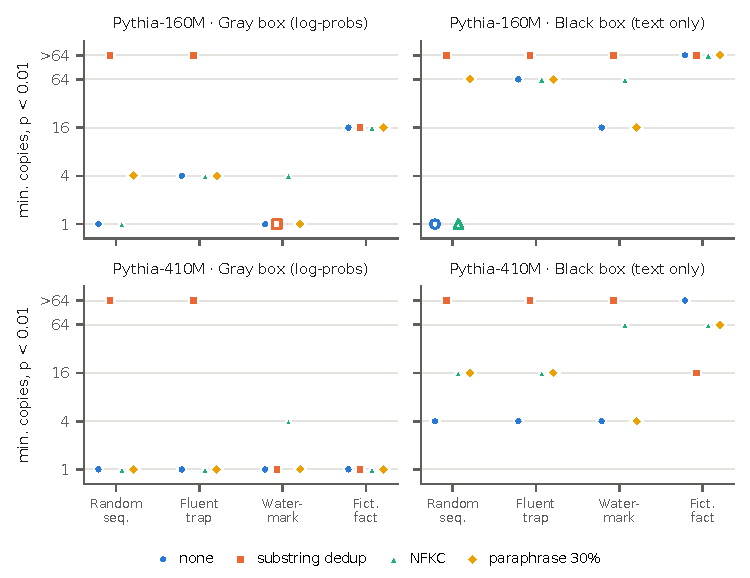
\includegraphics[width=\linewidth]{figs/fig1_dose.pdf}}{\fbox{Fig 1 pending}}
  \caption{Minimum number of planted copies at which the primary detector reaches $p<0.01$ (200 vs.\ 200
  canaries), per canary type and pipeline. ``$>$64'' = not detected at any dose.}
  \label{fig:dose}
\end{figure}

\textbf{How many copies?} \todo{RQ1 from Fig.~\ref{fig:dose} and Table~\ref{tab:bundle}.}

\begin{figure}[t]
  \centering
  \IfFileExists{figs/fig2_survival.pdf}{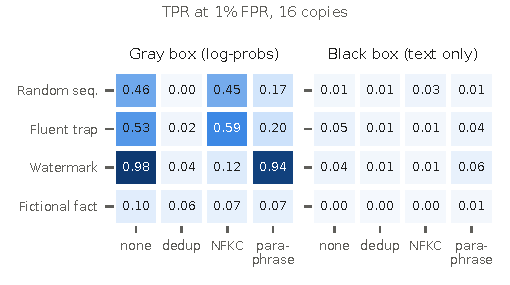
\includegraphics[width=\linewidth]{figs/fig2_survival.pdf}}{\fbox{Fig 2 pending}}
  \caption{TPR at 1\% FPR at 16 copies, per canary type (rows) and pipeline (columns), for each access level.}
  \label{fig:survival}
\end{figure}

\textbf{Does cleaning remove them?} \todo{RQ2 from Fig.~\ref{fig:survival} and the survival counts.}

\textbf{Is text-only access enough?} \todo{RQ3: gray vs.\ black panels.}

\begin{table}[t]
  \centering
  \caption{Minimum bundle size $m$ (members, with $m$ held-out controls) for which $\ge 80\%$ of resampled bundles
  give $p<0.01$, pipeline \emph{none}. ``--'' = not reached at $m=200$.}
  \label{tab:bundle}
  \small
  \IfFileExists{tables/table1_bundle.tex}{\begin{tabular}{lrrrrrrrr}
\toprule
 & \multicolumn{4}{c}{Gray box} & \multicolumn{4}{c}{Black box} \\
\cmidrule(lr){2-5}\cmidrule(lr){6-9}
Copies & 1 & 4 & 16 & 64 & 1 & 4 & 16 & 64 \\
\midrule
Random seq. & 200 & 100 & 10 & 10 & 200 & -- & -- & -- \\
Fluent trap & -- & 100 & 10 & 10 & -- & -- & -- & 50 \\
Watermark & 100 & 10 & 10 & 10 & -- & -- & 100 & 10 \\
Fictional fact & -- & -- & 100 & 10 & -- & -- & -- & -- \\
\midrule
\multicolumn{9}{l}{Clean base model: 0.0\% of 32 primary cells at $p<0.01$; re-split nulls: 1.1\% at $p<0.01$} \\
\bottomrule
\end{tabular}
}{Table 1 pending}
\end{table}

\begin{figure}[t]
  \centering
  \IfFileExists{figs/fig4_qq.pdf}{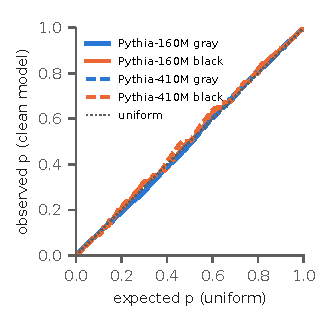
\includegraphics[width=0.45\linewidth]{figs/fig4_qq.pdf}}{\fbox{Fig 4 pending}}
  \caption{Clean base model: p-values from 200 random re-splits per cell against the uniform distribution.}
  \label{fig:qq}
\end{figure}

\textbf{Can we avoid false accusations?} \todo{RQ4 from Fig.~\ref{fig:qq} and the FPR line of Table~\ref{tab:bundle}.}

\begin{table}[t]
  \centering
  \caption{Canary scorecard. ``yes ($N$)'': detectable at $p<0.01$ from $N$ copies (gray box) after that pipeline.}
  \label{tab:scorecard}
  \small
  \IfFileExists{tables/scorecard.tex}{\begin{tabular}{lcccccc}
\toprule
Type & Min.\ copies & Dedup & NFKC & Paraphrase & Text-only & False acc. \\
\midrule
Random seq. & 1 & no & yes (1) & yes (4) & no & 0/8 \\
Fluent trap & 4 & no & yes (4) & yes (4) & yes (64) & 0/8 \\
Watermark & 1 & no & yes (4) & yes (1) & yes (16) & 0/8 \\
Fictional fact & 16 & yes (16) & yes (16) & yes (16) & no & 0/8 \\
\bottomrule
\end{tabular}
}{Scorecard pending}
\end{table}

\section{Discussion, limitations and ethics}
\textbf{Recommendation for writers.} If the developer's pipeline is unknown, plant \emph{fictional facts phrased
differently each time}, about 16 copies of each across 100 or more facts (or 64 copies across 10 facts). That is
provable at $p<0.01$ with log-probability access after deduplication, normalization and paraphrasing. Watermarks
are far cheaper (1--4 copies) but rely on the pipeline skipping Unicode normalization, and verbatim canaries rely on
it skipping substring deduplication. With text-only access, none of our designs is reliable at realistic copy
counts. Making facts extractable by questioning, not just memorized as sentences, is the open problem (and the target
for optimized canaries).

\textbf{Pre-registered vs.\ stable rule.} Running 32 tests per model at $\alpha=0.01$ produces occasional isolated
hits. We saw three, all at 1 copy (Fig.~\ref{fig:dose}, hollow markers). The scorecard therefore counts a dose
only if every higher dose is also detected. This rule is exploratory, and Fig.~\ref{fig:dose} reports the
pre-registered one.

\textbf{Limitations.} One model size (160M) and one seed per pipeline; larger models memorize more, so our copy
counts are likely conservative \todo{unless tier 1 adds 410M}. Fluent traps are template-generated rather than
sampled from an LM at a controlled perplexity. The paraphraser rewrites only the canary paragraph, not the
surrounding document. Commercial pipelines also filter by quality and apply post-training, which we do not study
in the main results.

\textbf{Ethics.} We audit only models we trained. The protocol is designed so that a creator cannot falsely accuse
a model that never saw their text: the false-positive rate is controlled by the randomized split, which we verify
on the clean base model.


\bibliographystyle{plainnat}
\bibliography{refs}

\appendix
\section{Pre-registration}\label{app:prereg}
The analysis plan (\texttt{docs/preregistration.md}) was committed to git before any canary-bearing model was
trained or scored. Commit \texttt{6ef2b5b} (Nov 10, 2026). The change log records two pre-result entries: the LR (App.~\ref{app:lr})
and 8 fictional entity names that also occur in the base corpus. Deviation after results: the ``stable'' minimum
dose used in the scorecard (Sec.~\ref{sec:results}), labelled exploratory. A third entry, written after the
160M results but before any 410M model was trained, fixes the 410M settings: same LR and analysis, batch
$2\times16$ for memory.

\section{Canary examples}\label{app:examples}
\todo{one example per type from data/canaries/mvr-v1.jsonl, rendered with zero-width characters shown as
$\langle$ZW$\rangle$.}

\section{Learning-rate selection}\label{app:lr}
Canary-free continued pretraining on 4.8M Wikipedia tokens; held-out loss on 50 unseen documents. bf16 autocast
inflated the loss and damaged the model, so the grid trains in tf32 and scores in fp32. Between the tf32 runs, the
larger LR was chosen, as pre-registered.

\begin{center}\small\IfFileExists{tables/app_lr.tex}{\begin{tabular}{lrrrr}
\toprule
Precision & LR & Held-out loss before & after & $\Delta$ \\
\midrule
tf32 & 1e-05 & 2.981 & 2.917 & -0.064 \\
tf32 & 3e-05 & 2.981 & 2.919 & -0.063 \\
bf16 & 1e-05 & 2.981 & 3.005 & +0.024 \\
bf16 & 3e-05 & 2.981 & 3.201 & +0.219 \\
bf16 & 1e-04 & 2.981 & 3.447 & +0.466 \\
\bottomrule
\end{tabular}
}{pending}\end{center}

\section{Numerical precision}\label{app:precision}
\todo{generated table: Pythia-160M loss in fp32 vs bf16 vs fp16 on 2048-token Wikipedia blocks, and on one short
sentence across CPU/A100/L40S.}

\section{Pipeline survival}\label{app:survival}
Planted copies still present (exact text; for fictional facts, entity and answer in the same document) after
each pipeline. The \emph{none} corpus has 82.5M tokens.

\begin{center}\small\setlength{\tabcolsep}{4pt}\IfFileExists{tables/app_survival.tex}{\begin{tabular}{lrrr}
\toprule
Type & substring dedup & NFKC & paraphrase 30\% \\
\midrule
Random seq. & 4.7\% (800/17,000) & 100.0\% (17,000/17,000) & 83.7\% (14,234/17,000) \\
Fluent trap & 4.5\% (766/17,000) & 100.0\% (17,000/17,000) & 69.5\% (11,823/17,000) \\
Watermark & 4.6\% (780/17,000) & 0.0\% (0/17,000) & 69.7\% (11,850/17,000) \\
Fictional fact & 99.9\% (16,983/17,000) & 100.0\% (17,000/17,000) & 99.9\% (16,987/17,000) \\
\midrule
Tokens & 77.5M & 82.1M & 82.3M \\
\bottomrule
\end{tabular}
}{pending}\end{center}

Per copy count. Under substring dedup, every canary keeps at most one copy, and all 1-copy random sequences
survive intact, so dedup and \emph{none} contain identical 1-copy canaries (Sec.~\ref{sec:results}).

\begin{center}\small\IfFileExists{tables/app_survival_dose.tex}{\begin{tabular}{lrrrr}
\toprule
Type & Copies & substring dedup & NFKC & paraphrase 30\% \\
\midrule
Random seq. & 1 & 200/200 & 200/200 & 166/200 \\
 & 4 & 200/800 & 800/800 & 658/800 \\
 & 16 & 200/3,200 & 3,200/3,200 & 2,661/3,200 \\
 & 64 & 200/12,800 & 12,800/12,800 & 10,749/12,800 \\
Fluent trap & 1 & 190/200 & 200/200 & 137/200 \\
 & 4 & 186/800 & 800/800 & 541/800 \\
 & 16 & 192/3,200 & 3,200/3,200 & 2,198/3,200 \\
 & 64 & 198/12,800 & 12,800/12,800 & 8,947/12,800 \\
Watermark & 1 & 190/200 & 0/200 & 138/200 \\
 & 4 & 192/800 & 0/800 & 563/800 \\
 & 16 & 199/3,200 & 0/3,200 & 2,232/3,200 \\
 & 64 & 199/12,800 & 0/12,800 & 8,917/12,800 \\
Fictional fact & 1 & 199/200 & 200/200 & 200/200 \\
 & 4 & 798/800 & 800/800 & 800/800 \\
 & 16 & 3,199/3,200 & 3,200/3,200 & 3,196/3,200 \\
 & 64 & 12,787/12,800 & 12,800/12,800 & 12,791/12,800 \\
\bottomrule
\end{tabular}
}{pending: run scripts/survival\_by\_dose.py}\end{center}

\section{All detectors}\label{app:all}
Primary detectors, every pipeline and dose (200 members vs.\ 200 non-members). Bold: $p<0.01$. Secondary
detectors are in \texttt{results/*/metrics.json}.

\paragraph{Pythia-160M.}
{\scriptsize\setlength{\tabcolsep}{4pt}\IfFileExists{tables/app_all_doses_p160m.tex}{\begin{tabular}{llrcccccc}
\toprule
 & & & \multicolumn{3}{c}{Gray box (loss)} & \multicolumn{3}{c}{Black box (completion)} \\
\cmidrule(lr){4-6}\cmidrule(lr){7-9}
Pipeline & Type & Copies & TPR & AUC & $p$ & TPR & AUC & $p$ \\
\midrule
none & Random seq. & 1 & 0.02 & 0.57 & \textbf{0.006} & 0.04 & 0.56 & \textbf{0.008} \\
 &  & 4 & 0.04 & 0.64 & \textbf{$2.9{\times}10^{-7}$} & 0.01 & 0.53 & 0.081 \\
 &  & 16 & 0.46 & 0.92 & \textbf{$3.2{\times}10^{-47}$} & 0.01 & 0.49 & 0.639 \\
 &  & 64 & 1.00 & 1.00 & \textbf{$2.4{\times}10^{-67}$} & 0.04 & 0.55 & 0.022 \\
 & Fluent trap & 1 & 0.04 & 0.55 & 0.048 & 0.00 & 0.51 & 0.330 \\
 &  & 4 & 0.01 & 0.65 & \textbf{$8.8{\times}10^{-8}$} & 0.01 & 0.47 & 0.831 \\
 &  & 16 & 0.53 & 0.95 & \textbf{$2.5{\times}10^{-55}$} & 0.05 & 0.51 & 0.347 \\
 &  & 64 & 1.00 & 1.00 & \textbf{$2.4{\times}10^{-67}$} & 0.18 & 0.73 & \textbf{$1.1{\times}10^{-15}$} \\
 & Watermark & 1 & 0.01 & 0.67 & \textbf{$4.0{\times}10^{-9}$} & 0.00 & 0.47 & 0.888 \\
 &  & 4 & 0.37 & 0.94 & \textbf{$1.5{\times}10^{-51}$} & 0.01 & 0.55 & 0.031 \\
 &  & 16 & 0.98 & 0.99 & \textbf{$3.1{\times}10^{-65}$} & 0.04 & 0.62 & \textbf{$1.7{\times}10^{-5}$} \\
 &  & 64 & 1.00 & 1.00 & \textbf{$2.4{\times}10^{-67}$} & 0.65 & 0.91 & \textbf{$1.9{\times}10^{-45}$} \\
 & Fictional fact & 1 & 0.01 & 0.57 & 0.011 & 0.00 & 0.51 & 0.191 \\
 &  & 4 & 0.01 & 0.52 & 0.298 & 0.00 & 0.52 & 0.063 \\
 &  & 16 & 0.10 & 0.66 & \textbf{$2.6{\times}10^{-8}$} & 0.00 & 0.51 & 0.064 \\
 &  & 64 & 0.20 & 0.88 & \textbf{$2.8{\times}10^{-40}$} & 0.00 & 0.51 & 0.251 \\
\midrule
substring dedup & Random seq. & 1 & 0.01 & 0.52 & 0.222 & 0.03 & 0.54 & 0.012 \\
 &  & 4 & 0.01 & 0.53 & 0.180 & 0.01 & 0.49 & 0.686 \\
 &  & 16 & 0.00 & 0.55 & 0.052 & 0.01 & 0.50 & 0.542 \\
 &  & 64 & 0.04 & 0.53 & 0.158 & 0.01 & 0.51 & 0.274 \\
 & Fluent trap & 1 & 0.01 & 0.56 & 0.026 & 0.01 & 0.50 & 0.439 \\
 &  & 4 & 0.00 & 0.52 & 0.261 & 0.01 & 0.48 & 0.743 \\
 &  & 16 & 0.02 & 0.50 & 0.453 & 0.01 & 0.54 & 0.093 \\
 &  & 64 & 0.02 & 0.54 & 0.066 & 0.04 & 0.50 & 0.546 \\
 & Watermark & 1 & 0.01 & 0.58 & \textbf{0.002} & 0.01 & 0.49 & 0.674 \\
 &  & 4 & 0.01 & 0.50 & 0.546 & 0.00 & 0.51 & 0.364 \\
 &  & 16 & 0.04 & 0.52 & 0.228 & 0.01 & 0.51 & 0.412 \\
 &  & 64 & 0.01 & 0.53 & 0.176 & 0.01 & 0.51 & 0.393 \\
 & Fictional fact & 1 & 0.00 & 0.57 & 0.011 & 0.01 & 0.50 & 0.332 \\
 &  & 4 & 0.01 & 0.52 & 0.273 & 0.00 & 0.51 & 0.121 \\
 &  & 16 & 0.06 & 0.67 & \textbf{$4.7{\times}10^{-9}$} & 0.00 & 0.51 & 0.157 \\
 &  & 64 & 0.17 & 0.88 & \textbf{$9.6{\times}10^{-41}$} & 0.00 & 0.52 & 0.033 \\
\midrule
NFKC & Random seq. & 1 & 0.01 & 0.57 & \textbf{0.008} & 0.01 & 0.58 & \textbf{$3.8{\times}10^{-4}$} \\
 &  & 4 & 0.11 & 0.65 & \textbf{$2.3{\times}10^{-7}$} & 0.01 & 0.48 & 0.743 \\
 &  & 16 & 0.45 & 0.91 & \textbf{$1.1{\times}10^{-45}$} & 0.03 & 0.51 & 0.365 \\
 &  & 64 & 1.00 & 1.00 & \textbf{$2.4{\times}10^{-67}$} & 0.12 & 0.59 & \textbf{$2.0{\times}10^{-4}$} \\
 & Fluent trap & 1 & 0.03 & 0.54 & 0.076 & 0.00 & 0.49 & 0.595 \\
 &  & 4 & 0.02 & 0.68 & \textbf{$6.8{\times}10^{-10}$} & 0.01 & 0.52 & 0.298 \\
 &  & 16 & 0.59 & 0.96 & \textbf{$1.7{\times}10^{-56}$} & 0.01 & 0.51 & 0.362 \\
 &  & 64 & 1.00 & 1.00 & \textbf{$2.4{\times}10^{-67}$} & 0.23 & 0.73 & \textbf{$5.9{\times}10^{-16}$} \\
 & Watermark & 1 & 0.01 & 0.50 & 0.449 & 0.01 & 0.53 & 0.178 \\
 &  & 4 & 0.01 & 0.60 & \textbf{$2.6{\times}10^{-4}$} & 0.01 & 0.47 & 0.880 \\
 &  & 16 & 0.12 & 0.70 & \textbf{$4.7{\times}10^{-12}$} & 0.01 & 0.51 & 0.416 \\
 &  & 64 & 0.33 & 0.80 & \textbf{$2.4{\times}10^{-25}$} & 0.12 & 0.63 & \textbf{$2.1{\times}10^{-6}$} \\
 & Fictional fact & 1 & 0.01 & 0.56 & 0.014 & 0.00 & 0.51 & 0.315 \\
 &  & 4 & 0.01 & 0.52 & 0.292 & 0.00 & 0.52 & 0.040 \\
 &  & 16 & 0.07 & 0.67 & \textbf{$5.2{\times}10^{-9}$} & 0.00 & 0.50 & 0.397 \\
 &  & 64 & 0.15 & 0.89 & \textbf{$1.5{\times}10^{-41}$} & 0.00 & 0.52 & 0.074 \\
\midrule
paraphrase 30% & Random seq. & 1 & 0.01 & 0.54 & 0.078 & 0.02 & 0.54 & 0.044 \\
 &  & 4 & 0.01 & 0.59 & \textbf{$6.6{\times}10^{-4}$} & 0.03 & 0.50 & 0.407 \\
 &  & 16 & 0.17 & 0.83 & \textbf{$3.5{\times}10^{-31}$} & 0.01 & 0.51 & 0.319 \\
 &  & 64 & 1.00 & 1.00 & \textbf{$2.4{\times}10^{-67}$} & 0.07 & 0.57 & \textbf{$9.6{\times}10^{-4}$} \\
 & Fluent trap & 1 & 0.01 & 0.50 & 0.514 & 0.01 & 0.52 & 0.244 \\
 &  & 4 & 0.03 & 0.58 & \textbf{0.002} & 0.02 & 0.48 & 0.786 \\
 &  & 16 & 0.20 & 0.81 & \textbf{$3.9{\times}10^{-27}$} & 0.04 & 0.52 & 0.278 \\
 &  & 64 & 0.99 & 1.00 & \textbf{$2.6{\times}10^{-67}$} & 0.06 & 0.60 & \textbf{$2.7{\times}10^{-4}$} \\
 & Watermark & 1 & 0.01 & 0.57 & \textbf{0.005} & 0.00 & 0.48 & 0.705 \\
 &  & 4 & 0.08 & 0.81 & \textbf{$8.2{\times}10^{-27}$} & 0.01 & 0.51 & 0.403 \\
 &  & 16 & 0.94 & 0.97 & \textbf{$2.3{\times}10^{-60}$} & 0.06 & 0.58 & \textbf{0.004} \\
 &  & 64 & 0.99 & 1.00 & \textbf{$3.0{\times}10^{-67}$} & 0.38 & 0.75 & \textbf{$5.4{\times}10^{-19}$} \\
 & Fictional fact & 1 & 0.01 & 0.56 & 0.017 & 0.01 & 0.50 & 0.496 \\
 &  & 4 & 0.00 & 0.51 & 0.366 & 0.00 & 0.51 & 0.241 \\
 &  & 16 & 0.07 & 0.67 & \textbf{$5.2{\times}10^{-9}$} & 0.01 & 0.50 & 0.496 \\
 &  & 64 & 0.15 & 0.88 & \textbf{$2.4{\times}10^{-40}$} & 0.00 & 0.50 & 0.506 \\
\bottomrule
\end{tabular}
}{pending}}

\paragraph{Pythia-410M.}
{\scriptsize\setlength{\tabcolsep}{4pt}\IfFileExists{tables/app_all_doses_p410m.tex}{\begin{tabular}{llrcccccc}
\toprule
 & & & \multicolumn{3}{c}{Gray box (loss)} & \multicolumn{3}{c}{Black box (completion)} \\
\cmidrule(lr){4-6}\cmidrule(lr){7-9}
Pipeline & Type & Copies & TPR & AUC & $p$ & TPR & AUC & $p$ \\
\midrule
none & Random seq. & 1 & 0.64 & 0.90 & \textbf{$1.4{\times}10^{-43}$} & 0.01 & 0.55 & 0.019 \\
 &  & 4 & 0.97 & 1.00 & \textbf{$1.3{\times}10^{-66}$} & 0.04 & 0.57 & \textbf{0.003} \\
 &  & 16 & 1.00 & 1.00 & \textbf{$2.4{\times}10^{-67}$} & 0.29 & 0.70 & \textbf{$9.1{\times}10^{-14}$} \\
 &  & 64 & 1.00 & 1.00 & \textbf{$2.4{\times}10^{-67}$} & 0.78 & 0.91 & \textbf{$6.2{\times}10^{-48}$} \\
 & Fluent trap & 1 & 0.09 & 0.74 & \textbf{$1.0{\times}10^{-16}$} & 0.01 & 0.53 & 0.124 \\
 &  & 4 & 0.71 & 0.97 & \textbf{$2.0{\times}10^{-59}$} & 0.07 & 0.57 & \textbf{0.009} \\
 &  & 16 & 1.00 & 1.00 & \textbf{$2.4{\times}10^{-67}$} & 0.35 & 0.76 & \textbf{$4.6{\times}10^{-19}$} \\
 &  & 64 & 1.00 & 1.00 & \textbf{$2.4{\times}10^{-67}$} & 0.93 & 0.98 & \textbf{$1.0{\times}10^{-63}$} \\
 & Watermark & 1 & 0.58 & 0.90 & \textbf{$2.0{\times}10^{-43}$} & 0.00 & 0.56 & 0.024 \\
 &  & 4 & 1.00 & 1.00 & \textbf{$2.4{\times}10^{-67}$} & 0.03 & 0.64 & \textbf{$1.1{\times}10^{-6}$} \\
 &  & 16 & 1.00 & 1.00 & \textbf{$2.4{\times}10^{-67}$} & 0.67 & 0.89 & \textbf{$3.2{\times}10^{-42}$} \\
 &  & 64 & 1.00 & 1.00 & \textbf{$2.4{\times}10^{-67}$} & 0.96 & 0.99 & \textbf{$1.3{\times}10^{-66}$} \\
 & Fictional fact & 1 & 0.00 & 0.61 & \textbf{$8.2{\times}10^{-5}$} & 0.01 & 0.50 & 0.419 \\
 &  & 4 & 0.01 & 0.62 & \textbf{$2.8{\times}10^{-5}$} & 0.01 & 0.51 & 0.323 \\
 &  & 16 & 0.17 & 0.83 & \textbf{$7.4{\times}10^{-30}$} & 0.01 & 0.53 & 0.017 \\
 &  & 64 & 0.64 & 0.98 & \textbf{$3.6{\times}10^{-61}$} & 0.02 & 0.53 & 0.016 \\
\midrule
substring dedup & Random seq. & 1 & 0.01 & 0.54 & 0.072 & 0.00 & 0.50 & 0.530 \\
 &  & 4 & 0.04 & 0.54 & 0.069 & 0.01 & 0.49 & 0.671 \\
 &  & 16 & 0.00 & 0.56 & 0.024 & 0.01 & 0.49 & 0.661 \\
 &  & 64 & 0.01 & 0.56 & 0.021 & 0.01 & 0.50 & 0.580 \\
 & Fluent trap & 1 & 0.02 & 0.54 & 0.088 & 0.01 & 0.49 & 0.613 \\
 &  & 4 & 0.00 & 0.54 & 0.076 & 0.01 & 0.48 & 0.784 \\
 &  & 16 & 0.04 & 0.55 & 0.042 & 0.00 & 0.50 & 0.558 \\
 &  & 64 & 0.02 & 0.56 & 0.014 & 0.01 & 0.50 & 0.486 \\
 & Watermark & 1 & 0.06 & 0.67 & \textbf{$9.0{\times}10^{-10}$} & 0.01 & 0.51 & 0.402 \\
 &  & 4 & 0.04 & 0.64 & \textbf{$3.0{\times}10^{-7}$} & 0.00 & 0.50 & 0.536 \\
 &  & 16 & 0.06 & 0.65 & \textbf{$1.2{\times}10^{-7}$} & 0.01 & 0.50 & 0.565 \\
 &  & 64 & 0.04 & 0.65 & \textbf{$1.1{\times}10^{-7}$} & 0.01 & 0.50 & 0.502 \\
 & Fictional fact & 1 & 0.01 & 0.61 & \textbf{$8.9{\times}10^{-5}$} & 0.01 & 0.50 & 0.409 \\
 &  & 4 & 0.04 & 0.62 & \textbf{$8.3{\times}10^{-6}$} & 0.00 & 0.50 & 0.501 \\
 &  & 16 & 0.18 & 0.84 & \textbf{$5.0{\times}10^{-32}$} & 0.01 & 0.53 & \textbf{0.009} \\
 &  & 64 & 0.62 & 0.98 & \textbf{$1.3{\times}10^{-62}$} & 0.02 & 0.55 & \textbf{$8.3{\times}10^{-4}$} \\
\midrule
NFKC & Random seq. & 1 & 0.58 & 0.88 & \textbf{$9.8{\times}10^{-41}$} & 0.01 & 0.54 & 0.047 \\
 &  & 4 & 0.90 & 0.98 & \textbf{$5.7{\times}10^{-63}$} & 0.01 & 0.56 & 0.011 \\
 &  & 16 & 1.00 & 1.00 & \textbf{$2.4{\times}10^{-67}$} & 0.14 & 0.69 & \textbf{$1.7{\times}10^{-12}$} \\
 &  & 64 & 1.00 & 1.00 & \textbf{$2.4{\times}10^{-67}$} & 0.79 & 0.92 & \textbf{$2.5{\times}10^{-49}$} \\
 & Fluent trap & 1 & 0.04 & 0.70 & \textbf{$7.3{\times}10^{-13}$} & 0.01 & 0.55 & 0.059 \\
 &  & 4 & 0.75 & 0.97 & \textbf{$4.8{\times}10^{-59}$} & 0.03 & 0.54 & 0.070 \\
 &  & 16 & 1.00 & 1.00 & \textbf{$2.4{\times}10^{-67}$} & 0.48 & 0.82 & \textbf{$1.1{\times}10^{-28}$} \\
 &  & 64 & 1.00 & 1.00 & \textbf{$2.4{\times}10^{-67}$} & 0.93 & 0.97 & \textbf{$1.3{\times}10^{-61}$} \\
 & Watermark & 1 & 0.04 & 0.56 & 0.027 & 0.01 & 0.52 & 0.200 \\
 &  & 4 & 0.12 & 0.77 & \textbf{$1.3{\times}10^{-20}$} & 0.00 & 0.51 & 0.386 \\
 &  & 16 & 0.62 & 0.93 & \textbf{$3.0{\times}10^{-51}$} & 0.07 & 0.54 & 0.078 \\
 &  & 64 & 0.85 & 0.99 & \textbf{$8.6{\times}10^{-64}$} & 0.23 & 0.71 & \textbf{$4.1{\times}10^{-13}$} \\
 & Fictional fact & 1 & 0.01 & 0.61 & \textbf{$7.3{\times}10^{-5}$} & 0.01 & 0.51 & 0.333 \\
 &  & 4 & 0.04 & 0.61 & \textbf{$5.4{\times}10^{-5}$} & 0.01 & 0.50 & 0.399 \\
 &  & 16 & 0.20 & 0.83 & \textbf{$1.1{\times}10^{-30}$} & 0.01 & 0.52 & 0.073 \\
 &  & 64 & 0.70 & 0.98 & \textbf{$1.9{\times}10^{-61}$} & 0.03 & 0.54 & \textbf{0.008} \\
\midrule
paraphrase 30% & Random seq. & 1 & 0.31 & 0.82 & \textbf{$1.3{\times}10^{-29}$} & 0.01 & 0.55 & 0.039 \\
 &  & 4 & 0.81 & 0.96 & \textbf{$1.4{\times}10^{-56}$} & 0.05 & 0.55 & 0.018 \\
 &  & 16 & 1.00 & 1.00 & \textbf{$2.4{\times}10^{-67}$} & 0.19 & 0.65 & \textbf{$3.2{\times}10^{-8}$} \\
 &  & 64 & 1.00 & 1.00 & \textbf{$2.4{\times}10^{-67}$} & 0.74 & 0.88 & \textbf{$1.5{\times}10^{-42}$} \\
 & Fluent trap & 1 & 0.04 & 0.61 & \textbf{$9.1{\times}10^{-5}$} & 0.01 & 0.51 & 0.350 \\
 &  & 4 & 0.19 & 0.84 & \textbf{$8.0{\times}10^{-33}$} & 0.01 & 0.52 & 0.290 \\
 &  & 16 & 0.99 & 1.00 & \textbf{$2.8{\times}10^{-67}$} & 0.14 & 0.63 & \textbf{$4.1{\times}10^{-6}$} \\
 &  & 64 & 1.00 & 1.00 & \textbf{$2.4{\times}10^{-67}$} & 0.80 & 0.93 & \textbf{$4.7{\times}10^{-51}$} \\
 & Watermark & 1 & 0.30 & 0.73 & \textbf{$2.3{\times}10^{-16}$} & 0.00 & 0.55 & 0.051 \\
 &  & 4 & 0.87 & 0.98 & \textbf{$9.4{\times}10^{-63}$} & 0.02 & 0.58 & \textbf{0.004} \\
 &  & 16 & 1.00 & 1.00 & \textbf{$2.4{\times}10^{-67}$} & 0.39 & 0.75 & \textbf{$9.0{\times}10^{-19}$} \\
 &  & 64 & 1.00 & 1.00 & \textbf{$2.4{\times}10^{-67}$} & 0.97 & 1.00 & \textbf{$7.1{\times}10^{-68}$} \\
 & Fictional fact & 1 & 0.01 & 0.60 & \textbf{$3.3{\times}10^{-4}$} & 0.01 & 0.51 & 0.147 \\
 &  & 4 & 0.03 & 0.61 & \textbf{$5.2{\times}10^{-5}$} & 0.01 & 0.51 & 0.258 \\
 &  & 16 & 0.12 & 0.81 & \textbf{$1.4{\times}10^{-27}$} & 0.01 & 0.52 & 0.057 \\
 &  & 64 & 0.68 & 0.97 & \textbf{$5.1{\times}10^{-59}$} & 0.01 & 0.54 & \textbf{0.006} \\
\bottomrule
\end{tabular}
}{pending}}

\section{False-positive check}\label{app:qq}
\begin{center}
  \IfFileExists{figs/fig4_qq.pdf}{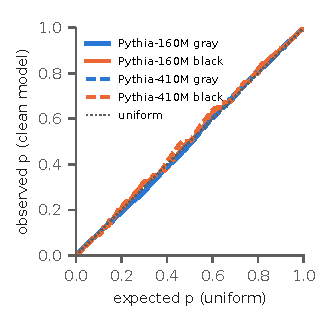
\includegraphics[width=0.4\linewidth]{figs/fig4_qq.pdf}}{\fbox{Fig 4 pending}}
  \captionof{figure}{Clean base models: p-values from 200 random re-splits per cell against the uniform
  distribution, for both primary detectors and both model sizes.}\label{fig:qq}
\end{center}


\end{document}
